\documentclass[mnsc, blindrev]{informs3}
\usepackage{mystyle}
\OneAndAHalfSpacedXI
\usepackage{natbib}
 \bibpunct[, ]{(}{)}{,}{a}{}{,}%
 \def\bibfont{\small}%
 \def\bibsep{\smallskipamount}%
 \def\bibhang{24pt}%
 \def\newblock{\ }%
 \def\BIBand{and}%


\TheoremsNumberedThrough     % Preferred (Theorem 1, Lemma 1, Theorem 2)

\ECRepeatTheorems

\EquationsNumberedThrough    % Default: (1), (2), ...

\MANUSCRIPTNO{MS-0001-1922.65}

\newcommand{\arpit}{\color{red}}
\newcommand{\nolan}{\color{blue}}

%\newcommand{\argmin}{\arg\!\min}
%\newcommand{\argmax}{\arg\!\max}

% Definitions of Math Symbols
\def\a{\alpha}
\def\b{\beta}
\def\t{\tau}
\def\th{\theta}
\def\r{\rho}
\def\eps{\epsilon}
\def\d{\delta}
\def\ve{\varepsilon}
\def\D{\Delta}
\def\k{\kappa}
\def\L{\Lambda}
\def\G{\Gamma}
\def\Th{\Theta}
\def\l{\lambda}
\def\m{\mu}
\def\et{\eta}
\def\g{\gamma}

\def\ie{i.e.}
\def\eg{e.g.}

\def\beq{\begin {equation}}
\def\eeq{\end {equation}}
\def\beqar{\begin {eqnarray*}}
\def\eeqar{\end {eqnarray*}}
\def\beqarn{\begin {eqnarray}}
\def\eeqarn{\end {eqnarray}}
%\def\end{proof}{\endproof}
                 
\providecommand{\abs}[1]{\lvert#1\rvert}

%\newtheorem{fact}{Fact}[section]
%\newtheorem{rules}{Rule}[section]
%\newtheorem{theorem}{Theorem}[section]
%\newtheorem{remark}{Remark}
%\newtheorem{proposition}{Proposition}
%\newtheorem{corollary}{Corollary}[section]
%\newenvironment{proofof}[1]{\noindent {\em Proof of #1.  }}{\hfill$\Box$}
%\newtheorem{definition}{Definition}[section]
%\newtheorem{lemma}{Lemma}[section]
%\newtheorem{claim}{Claim}
%\newtheorem{conjecture}{Conjecture}

\def \imp {\rightarrow}
\def \qed {\hfill $\Box$}
\def \R {{\mathbb R}}
\def \sR {{\mathcal R}}
\def \eps {\varepsilon}
\def \N {{\mathbb N}}
\def \Z {{\mathbb Z}}
\newcommand{\ignore}[1]{}
\newcommand{\fignore}[1]{#1}
\def \poly { \text{\rm poly~} }
\def \polylog { \text{\rm polylog~} }
\def\th{{\text{\rm th}}}

\newcommand{\expect}{\mathbb{E}}
\newcommand{\indicate}{\mathds{1}}
\newcommand{\circE}{\overset{\circ}{E'}}
\newcommand{\prob}{\mathbb{P}}
\newcommand{\real}{\mathbb{R}}
\newcommand{\calG}{\mathcal{G}}
\newcommand{\calF}{\mathcal{F}}
\newcommand{\calM}{\mathcal{M}}
\newcommand{\calN}{\mathcal{N}}
\newcommand{\calP}{\mathcal{P}}
\newcommand{\calS}{\mathcal{S}}
\newcommand{\calC}{\mathcal{C}}
\newcommand{\calT}{\mathcal{T}}
\newcommand{\calD}{\mathcal{D}}
\newcommand{\calU}{\mathcal{U}}
\newcommand{\cd}{\mathcal{d}}

\newcommand{\rms}{r^{\min}_s}
\newcommand{\rmsp}{r^{\min}_{s'}}
\newcommand{\ems}{E^{\min}_s}
\newcommand{\emsp}{E^{\min}_{s'}}
\newcommand{\vms}{V^{\min}_s}
\newcommand{\vmsp}{V^{\min}_{s'}}
\newcommand{\vxs}{V^X_s}
\newcommand{\vxsp}{V^X_{s'}}
\newcommand{\vis}{V^{\text{int}}_s}
\newcommand{\visp}{V^{\text{int}}_{s'}}

\newcommand{\bint}{\mathbf{int}}

\newcommand{\ZE}{{\sf ZE}}
\newcommand{\IX}{{\sf IX}}
\newcommand{\DP}{{\sf DP}}
\newcommand{\TV}{{\sf TV}}
\newcommand{\TP}{{\sf TP}}
\newcommand{\TD}{{\sf TD}}
\newcommand{\DT}{{\sf DT}}
\newcommand{\EU}{{\sf EU}}



\newcommand{\ER}{Erd\"{o}s-R\'{e}nyi}          
\newcommand{\BetaDist}{\mathit{Beta}}    

\newcommand{\strats}{\calS}
\newcommand{\numStrats}{m}
\newcommand{\eqcand}{\sigma}


\begin{document}

\RUNTITLE{Optimal Frequency Reward Program}
\TITLE{Design of an Optimal Frequency Reward Program in the Face of Competition}

\ARTICLEAUTHORS{%
\AUTHOR{Arpit Goel}
\AFF{Department of Management Science and Engineering, Stanford University, Stanford, CA, 94305, \EMAIL{argoel@stanford.edu}}
\AUTHOR{Nolan Skochdopole}
\AFF{Institute for Computational and Mathematical Engineering, Stanford University, Stanford, CA, 94305, \EMAIL{naskoch@stanford.edu}}
}

\ABSTRACT{%
We optimize the design of a frequency reward program against traditional pricing in a competitive duopoly, where customers measure their utility in rational economic terms.
We assume two kinds of customers: myopic and strategic (\cite{yilmaz2016upgrade}). 
Every customer has a prior loyalty bias (\cite{fader1993excess}) toward the reward program merchant, a parameter drawn from a known distribution, indicating an additional probability of choosing the reward program merchant over the traditional pricing merchant.
Under this model, we characterize the customer behavior: the loyalty bias increases the switching costs (\cite{klemperer1995competition}) of strategic customers until a tipping point, after which they strictly prefer and adopt the reward program merchant. 
Subsequently, we optimize the reward parameters to maximize the revenue objective of the reward program merchant.
We show that under mild assumptions, the optimal parameters for the reward program design to maximize the revenue objective, correspond exactly to minimizing the tipping point of customers, and are independent of the customer population parameters. 
Moreover, we characterize the conditions for the reward program to be better when the loyalty bias distribution is uniform - a minimum fraction of population needs to be strategic, and the loyalty bias needs to be in an optimal range.
If the bias is high, the reward program creates loss in revenues, as customers effectively gain rewards for ``free'', whereas a low value of bias leads to loss in market share to the competing merchant.
In short, if a merchant can estimate the customer population parameters, our framework and results provide theoretical guarantees on the pros and cons of running a reward program against traditional pricing.

}

\KEYWORDS{loyalty reward, marketing, revenue management, customer choice} \HISTORY{This paper was
first submitted on February 12, 2017.}

\maketitle
\section{Introduction}
\label{sec:intro}
Loyalty programs constitute a huge market in consumer retail and are a major source of revenue for many low margin businesses.
Over 48 billion dollars in perceived value of rewards is issued in the United States alone every year, with every household having over 19 loyalty memberships on average (\cite{berry2013loyalty}).
This market constitutes credit cards, hotel and airline reward programs, and more recently even restaurants, grocery and retail stores.
In addition to possibly increasing their market share, these reward programs provide many benefits to the merchants -- for instance, user identification for firms having multiple purchase channels; increase in sales due to referrals; personalized price discrimination and product recommendations, to name a few (\cite{ryu2007penny}).
There are many examples of popular reward programs -- Starbucks allows members to earn ``stars'' on purchases which can be redeemed for free coffee, Bloomingdale's offers \$25 reward for around \$1500 spent in their store, and Target offers a 5\% cashback on all purchases (\cite{cvs2015target}).
Though forming a big component of the market, there is little scientific understanding about the design of loyalty reward programs. We aim to address this gap with our research.

One popular form of loyalty reward programs is \emph{frequency reward programs}, where customers earn \emph{points} as currency over spendings with merchants and are able to redeem these points for dollar valued rewards after achieving certain threshold point collections.
There is extant literature on characterizing customer behavior toward frequency reward programs.
Most of the literature is empirical in nature, and relies on psychological behavioral patterns among customers, as opposed to rational economic decision making (\cite{kivetz2006goal,dreze2004using,gao2014influence}) .
In this paper, we consider a competitive duopoly of two merchants where one merchant offers a frequency reward program and the other offers traditional pricing with discounts.
Though revenue management literature often deals with dynamic pricing of products, many retail merchants offering rewards often pre-commit to their prices. 
We assume that both merchants commit to their product pricing apriori and characterize a novel model of customer choice where customers measure their utilities in rational economic terms.
In addition, we investigate the direct effects on the revenue objective and characterize the optimal reward design choice for the merchant offering the frequency reward program, based on different customer populations.
Specifically, we answer the following question: how should the merchant decide the optimal thresholds and dollar value of rewards to optimize for its revenue share from the participating customer population.
One important constraint we impose is that the merchant has to choose a \emph{one design fits all} reward program for the entire participating customer population and is not allowed to personalize the program for different customer segments.

This is how the remaining paper is structured. First, we will describe some related work. Then we will give an overview of our model and results. 
In Section~\ref{sec:model} we will describe our model in technical detail followed by the main results in Section~\ref{sec:results}. 
We will conclude with a short discussion on future work in Section~\ref{sec:conc}.

\subsection{Related Work}
Three popular psychological constructs have been used to explain customer choice dynamics toward reward programs -- Goal Gradient Hypothesis, Medium Maximization, and Tipping Point Dynamics.
\cite{kivetz2006goal} conducted an empirical study observing an acceleration in the number of purchases by customers as they approached the reward, \ie, as customers accumulated reward points to reach closer to achieving the reward, their effort invested toward gaining more points increased. 
The authors attributed this behavior to Goal Gradient Hypothesis (\cite{hull1932goal}). 
This behavior is also very prevalent in online badge systems, such as those on Stackoverflow; recently, mathematical models relying on rational user behavior have been developed that explain this phenomenon (\cite{leskovec2013steering}).
\cite{stourm2015stockpiling, dreze2004using} observed that customers often stockpiled reward points even when there were economic incentives against the collection of points. They attributed this behavior to Medium Maximization -- customers often treated collecting reward points as a goal itself just like collecting stamps as opposed to connecting reward points with economic incentives.
Correspondingly, they introduced a new model where customers had different ``mental accounts'' and utility functions for points and cash.
\cite{gao2014influence} observed via experimentation that customers often collect reward points for exogenous reasons until they accumulate a threshold amount, after which they start investing effort toward the collection process itself.
That is, customers build up switching costs (\cite{klemperer1995competition}) before fully adopting the reward program, and sometimes this switching cost is created due to reasons exogenous to rational economic incentives.
They referred to this behavior as the Tipping Point Effect.

A large body of literature investigates the switching costs customers face within a competitive duopoly framework -- see \cite{villas2015short} for a short survey.
Our model is closest in spirit to that of \cite{hartmann2008frequency} and \cite{kopalle2001economic}.
Both papers are empirical in nature and model a competitive duopoly where customers maximize their long term discounted utility.
\cite{hartmann2008frequency} argue that less frequent buyers face higher switching costs as they are more likely to be affected by reward redemption deadlines, whereas frequent buyers redeem rewards easily and do not face substantial switching costs. 
They do not model how customers build up switching costs, but only argue what happens when customers are close to achieving a reward.
\cite{kopalle2001economic} discuss dynamic competition between two merchants deciding whether to offer a reward program or traditional pricing and model this decision problem as a two stage game: first merchants decide whether to offer a reward program or traditional pricing and then they decide their prices. 
Using simulations, depending on customer parameters in the model, they characterize the conditions for when it is better to offer a reward program versus traditional pricing.
We on the other hand model a multi-period problem where the customer behavior is characterized using a complete dynamic program, and mathematically analyze our model.
We make two modeling assumptions: first is an exogenous visit probability bias toward the reward program merchant which can be attributed to \emph{excess loyalty} -- customers often build up higher brand preference toward the merchant offering a reward program (\cite{fader1993excess, sharp1997loyalty}); 
and second, a look-ahead factor for customers, which indicates how far into the future customers can perceive the rewards (\cite{liu2007long,lewis2004influence}).
Our results on customer choice dynamics intuitively look similar to some of those obtained in the above mentioned body of literature.
But more importantly, we model and optimize the revenue objective of the merchant, characterizing an optimal reward program design for maximizing expected revenue.


\subsection{Our Contributions}
We make both modeling and analytical contributions along the following directions:

\subsubsection{Competitive Duopoly Setup}
We model a competitive duopoly of two merchants, one of them offering a frequency reward program and the other offering traditional pricing.
Both merchants sell an identical good at fixed precommitted prices.
The reward program merchant sells the good at a higher price.
Customers are drawn from a known population distribution and they measure their utilities in rational economic terms, \ie, they make their purchase decisions to maximize long term discounted rewards.
The discount factor is the time value of money, and is constant for all customers.
Every customer makes a purchase everyday from either of the two merchants.
With each purchase from the reward program merchant, customer gains some fixed number of points, and on achieving the reward redemption threshold, (s)he immediately gains the reward value as a dollar cashback.

\subsubsection{Customer Parameters}
Each customer has two important parameters drawn from the known population distribution: first a visit probability bias with which (s)he purchases the good from the reward program merchant for reasons exogenous to utility maximization, and second a look-ahead factor that controls how far into the future the customer can perceive the rewards.
The visit probability bias toward the reward program merchant can be attributed to \emph{excess loyalty} which has been argued as a important parameter for the success of any reward program, or it can be attributed to price insensitivity of the customer; whenever the customer is price insensitive, (s)he strictly prefers to purchase from the reward program merchant as (s)he gains points redeemable for rewards in the future.
There are many possible reasons for customers' price insensitivity: the reward program merchant could be offering some other monopoly products, or the customer might be getting reimbursed for some purchases as part of corporate perks (eg: corporate travel).
As an effect, this visit probability bias controls how frequently the customers' points increase even when (s)he does not actively choose to make purchases from the reward program merchant.
The look-ahead parameter affects the customer behavior dynamics as follows: if the reward is farther than the customer's look-ahead parameter, (s)he is unable to register the future value of that reward and take it into consideration while maximizing long term utility.
Both these parameters can be attributed to bounded rationality of customers and have been argued to be important factors toward customer choice dynamics.


\subsubsection{Customer Choice Dynamics}
We formulate the customer choice dynamics as a dynamic program with the state being the number of points collected from the reward program merchant.
When the customer does not make biased visits to the reward program merchant, she chooses the merchant maximizing her long term utility: comparing the immediate utility by purchasing the good at cheaper price and the long term utility of waiting and receiving the time discounted reward.
The solution to the customer's dynamic program gives conditions for the existence and achievability of a phase transition: a points threshold before which the customer visits the merchant offering rewards only due to the visit probability bias, and after which (s)he always visits the merchant offering rewards till receiving the reward.
We show that this phase transition point has the following dependencies:
\begin{enumerate}
\item It decreases with increase in the look-ahead parameter, \ie, if the customer can perceive rewards longer into the future, the phase transition for the customer occurs sooner.
\item It decreases with increase in the reward value, and decreases with increase in points threshold required to redeem the reward. 
\item It increases with the discount value that the traditional pricing merchant provides, \ie, the cheaper the product from the second merchant, the farther is the phase transition point. 
\item With respect to the discount factor there is a unique minimizer for the phase transition point. That is, if customers are highly patient, then maximizing their long term utility leads them to redeem rewards only due to exogenous visit bias.
And if they are very less patient, they strictly prefer immediate discount over future rewards.
\end{enumerate}

We define the ``influence zone'' as the ratio of the distance to the phase transition  point and the total distance to the reward.
This is effectively the fraction of total purchases until reward redemption that the customer needs to make due to exogenous visit bias to adopt the reward program for future purchases.
Merchants often give bonus miles or points to their customers, mainly to increase the switching cost of customers and push them to adopt the reward program.
The influence zone as we defined is the point till such external promotions are required.
We optimize over this influence zone and show that the optimal distance to the reward has a very intuitive form which corresponds closely to practically observed values for the reward distance.

In short, these results verify that our model is in coherence with the different psychological constructs as discussed in the related work section: purchase acceleration closer to reward redemption and a tipping point before which purchases are only due to exogenous visit bias.

\subsubsection{Reward Program Design}
After characterizing the customer behavior dynamics in our model, we optimize over the long run revenues that the reward program merchant achieves.
We provide a framework for optimizing the parameters for the reward program merchant to maximize its revenue objective.
We then look at a specific simplified case of proportional promotion budgeting: the reward offered by the reward program merchant is proportional to the product of the distance to the reward and the discount provided by the traditional pricing merchant.
We show that under proportional promotion budgeting the optimal distance to reward for maximizing the revenue objective of the reward program merchant is independent of the customer parameters and is close to the real world obtained cashback percentage amounts.
In addition, optimizing the revenue objective gives the same optimal distance to reward as optimizing the influence zone as defined above.
Moreover, we characterize the conditions in terms of the customer parameters for when the revenue objective of the reward program merchant is better than the traditional pricing merchant and when it is better for the reward program merchant to offer a reward versus not offering any reward.
We show that for the reward program to be effective under both the above conditions, a minimum threshold fraction of customers must be ``forward-looking''.
And there is a range of values of the exogenous visit probability bias between $0$ and $1$ corresponding to the fraction of ``forward-looking'' customers for the reward program to be strictly better for the merchant. 


\section{Model}
\label{sec:model}
We index the two competing merchants selling identical goods as $A$ and $B$.
Without loss of generality we assume that $A$ sells the good for a price of $1$ dollar while $B$ sells it for $1-v$ dollars, \ie, $B$ offers a discount of $v$ dollars\footnote{\arpit Add footnote that this assumption can be made for arbitrary pricing, and our results extend}. 
Merchant $A$ additionally offers a reward of value $R$ dollars to a customer after (s)he makes $k$ purchases at $A$. 
We only investigate the case that we refer to as ``proportional promotion budgeting'', wherein this reward $R$ is proportional to the product of the distance to the reward $k$ and the discount $v$ provided by $B$;
that is, $R = \alpha k v$.
The merchant optimizes over both $k$ and $\alpha$.
This assumption imposes the constraint that the reward offered by the merchant is linearly dependent to the distance to reward. {\nolan Add justification for proportional budgeting here - linear reward scheme source.}

\subsection{Customer Behavior Model}
We assume customers purchase the item from either $A$ or $B$ everyday, \ie, we ignore the heterogeneity in frequency of purchases among the customers in our model and leave it for future work.
We assume customers have a linear homogenous utility in price: at price $q$ the utility is $\nu(q) = 1-q$. 
This reduces to customers getting an immediate utility of $0$ from $A$ and $v$ from $B$.
All customers have the same time value of money as a discount factor of $\beta$ lying between $0$ and $1$.

We denote a customer's visit probability bias and the look-ahead parameter with $\lambda$ and $t$ respectively. 
That is with probability $\lambda$, (s)he purchases from $A$ due to externalities and perceives a future reward only if it is within $t$ purchases away. 
This $\lambda$ for a customer is drawn from a distribution $f$ with support between $[0,1]$.
In this paper, we focus on a simple threshold distribution for the look-ahead parameter $t$: 

\begin{equation*}
  t=\begin{cases}
    t_1, & \text{wp } p,\\
    0, & \text{wp } 1-p.
  \end{cases}
\end{equation*}

The above distribution intuitively means that the customers are either myopic and focus only on immediate rewards or are strategic and can perceive long term utility (we assume $t_1$ is large).
We leave other parametrizations of this look-ahead parameter for future work.
We model the customer's decision problem as a dynamic problem. We index the number of purchases the customer makes from $A$ until the reward by $i$, for $0 \leq i \leq k-1$, and we refer a customer to be in state $i$ after having made $i$ purchases from $A$. At state $i$, the customer has two possibilities:
\begin{enumerate}
\item
With probability $\lambda$, the customer must visit $A$, and she is now in state $i+1$.
\item
With probability $1-\lambda$, the customer may purchase from $B$ for an immediate utility $v$ and remain in state $i$ or purchase from $A$ for no immediate utility but move to state $i+1$.
\end{enumerate}

Let $V(i)$ denote the long term expected reward at state $i$. Then we model the decision problem as the following dynamic program.
\begin{align*}
& V(i) = \lambda \beta V(i+1) + (1-\lambda)\max\{v+\beta V(i),\beta V(i+1) \} \mbox{ for } 0\leq i \leq k-1 \\
& V(k) = R
\end{align*}

We show that the decision process exhibits a phase transition; that is prior to some state, the customer purchases from $A$ only if (s)he must do so exogenously but after that state, (s)he always decides to purchase from $A$. 
This phase transition point is independent of $\lambda$, and depends only on $t$, among the variable customer parameters.
Hence we represent this phase transition point as $i_0(t)$.

\subsection{Merchant Objective}
Given the above model of customer dynamics, we define the revenue objectives of $A$ and $B$, where $A$ chooses its reward parameters and $B$ is non strategic. 
We define the rate of revenue for a merchant from a customer as the expected time averaged revenue that the merchant receives within the customer's lifetime.
For simplification, we assume merchants do not discount future revenues.
As described above, a customer's dynamics are cyclic after each reward cycle.
Thus the lifetime dynamics of customer behavior is a regenerative process with independent and identically distributed reward cycle lengths.
Let $RoR_A(c)$ and $RoR_B(c)$ denote the expected rate of revenues for $A$ and $B$ respectively from a customer $c$'s lifetime.
Let $\tau(t, \lambda)$ denote the total number of purchases the customer makes before reaching the phase transition point $i_0(t)$.
Then the length of the reward cycle (or total number of purchases the customer makes before receiving the reward) is $\tau(t, \lambda) + k - i_0(t)$, because after the phase transition (s)he makes all purchases from $A$ only until hitting the reward.
In this cycle the number of visits that the customer makes to $A$ is $k$, and to $B$ is $\tau(t,\lambda) - i_0(t)$.
The revenue that $A$ earns in one such cycle is $k-R$ and the revenue that $B$ earns is $(1-v)(\tau(t,\lambda) - i_0(t))$.
Thus the rate of revenues for $A$ and $B$ from the customer $c$ are as follows:
\beq
RoR_A(c) = \underset{\tau, t, \lambda}E\left[\frac{k-R}{\tau(t,\lambda) + k - i_0(t)}\right]\notag
\eeq
\beq
RoR_B(c) = \underset{\tau, t, \lambda}E\left[\frac{(\tau(t,\lambda) - i_0(t))(1-v)}{\tau(t,\lambda) + k - i_0(t)}\right]\notag
\eeq

Since the process for a single customer is regenerative, using the reward renewal theorem (\cite{10.2307/1426216}), we can take the expectation over the cycle length inside the numerator and denominator respectively.
Note that $\underset{\tau, t, \lambda}E[\tau(t,\lambda)] = \frac{i_0(t)}{\lambda}$ as before reaching the phase transition point, with probability $\lambda$, the number of purchases by the customer from $A$ increases by $1$ and with probability $1-\lambda$ it stays constant.
Then taking the expectation over the customer population the overall rate of revenues for both $A$ and $B$ are as follows:

\beq
RoR_A = \underset{\lambda, t}E\left[\frac{k-R}{i_0(t)/\lambda + k - i_0(t)}\right]
\eeq

\beq
RoR_B = \underset{\lambda, t}E\left[\frac{(i_0(t)\lambda - i_0(t))(1-v)}{i_0(t)/\lambda + k - i_0(t)}\right]
\eeq


\section{Results}
\label{sec:results}
\subsection{Customer Choice Dynamics}
We first show that every customer exhibits the following behavior: until (s)he reaches the phase transition point $i_0(t)$, she purchases from $A$ only due to the exogeneity paramater, and after that (s)he always purchases from $A$ till she receives the reward.
This behavior is cyclic, and repeats after every reward redemption.

\begin{lemma} $V(i)$ is an increasing function in $i$ if the following condition holds:
\begin{equation}
R > \frac{(1-\lambda)v}{1-\beta}
\end{equation}
And further, $V(i)$ can be evaluated as:
\begin{equation}
V(i) = \max\left\{ \frac{\lambda \beta V(i+1)+(1-\lambda)v}{1-(1-\lambda)\beta}, \beta V(i+1) \right\}
\end{equation}
\end{lemma}

\proof
First we show that $V(i)$ is an increasing function in $i$ by induction. We first show that if the condition above is satisfied, $V(k-1) < V(k) = R$. Suppose not, so $V(i) \geq R$. Then we have:
\begin{align*}
V(k-1) &= \lambda \beta V(k) + (1-\lambda)(v+\beta V(k-1)) \\
&= \frac{\lambda \beta R + (1-\lambda)v}{1-(1-\lambda)\beta} \\
&< \frac{\lambda \beta R + (1-\beta)R}{1-(1-\lambda)\beta} \\
&= \frac{R(1-(1-\lambda)\beta)}{1-(1-\lambda)\beta} = R
\end{align*}
But this is a contradiction, so $V(k-1) < V(k)$. Now assume $V(i+1) < V(i+2)$ for some $i < k-2$, we will show that this implies $V(i) < V(i+1)$. Suppose not, so $V(i) \geq V(i+1)$. As we did before we may upper bound $V(i)$.
\begin{align*}
V(i) &= \lambda \beta V(i+1) + (1-\lambda)(v+\beta V(i)) \\
&\leq (1-\lambda)v + \beta V(i) \\
\iff V(i) &\leq \frac{(1-\lambda)v}{1-\beta}
\end{align*}
But because $V(i+1) < V(i+2)$, we may lower bound $V(i+1)$.
\begin{align*}
V(i+1) &\geq \lambda \beta V(i+2) + (1-\lambda)(v+\beta V(i+1)) \\
&= (1-\lambda)v + (1-\lambda)\beta V(i+1) + \lambda \beta V(i+2) \\
&> (1-\lambda)+\beta V(i+1) \\
\iff V(i+1) &> \frac{(1-\lambda)v}{1-\beta}
\end{align*}
Again, we have a contradiction, so $V(i) < V(i+1)$, and $V(i)$ is an increasing function in $i$. Now we prove the second claim. We have the following:
\begin{align*}
V(i) &= \lambda \beta V(i+1) + (1-\lambda)\max\{v +\beta V(i), \beta V(i+1) \} \\
&= \max\{\lambda \beta V(i+1) + (1-\lambda)(v+\beta V(i)), \beta V(i+1) \}
\end{align*}

Assuming $V(i)$ is the left term in the above maximum, we may solve the equation for that term.
\begin{gather*}
V(i) = \lambda \beta V(i+1) + (1-\lambda)(v+\beta V(i)) \\
(1-(1-\lambda)\beta) V(i) = \lambda \beta V(i+1) + (1-\lambda)v \\
V(i) = \frac{\lambda \beta V(i+1) + (1-\lambda)v}{1-(1-\lambda)\beta}
\end{gather*}
And we get our claim.
\endproof

Now if the expected reward of the customer increases with the number of purchases made from $A$, we expect that at some number of purchases it becomes profitable for the customer to choose to purchase from $A$ as opposed to $B$.
We characterize this phase transition point in the following theorem.

\begin{theorem} Suppose $V(i)$ is an increasing function in $i$ and consider a customer with look-ahead parameter $t$. A phase transition occurs after (s)he makes $i_0(t)$ visits to firm $A$, where $i_0(t)$ is given by:
\begin{equation}
  i_0(t)=\begin{cases}
    k-\Delta \equiv i_0, & \text{if $t \geq \Delta$}.\\
    k-t, & \text{otherwise}.
  \end{cases}
\end{equation}
with 
\begin{align}
\Delta &= \left\lfloor \log_{\beta}\left(\frac{v}{R(1-\beta)}\right)\right\rfloor
\end{align}
\end{theorem}

\proof
First we solve for the condition on $V(i+1)$ for us to choose firm $A$ over $B$ willingly.
\begin{gather*}
\beta V(i+1) > \frac{\lambda \beta V(i+1) + (1-\lambda)v}{1-(1-\lambda)\beta} \\
\iff \beta V(i+1) \left(1-\frac{\lambda}{1-(1-\lambda)\beta} \right) > \left(\frac{1-\lambda}{1-(1-\lambda)\beta} \right) v \\
\iff \beta V(i+1) \left(\frac{1-(1-\lambda)\beta -\lambda}{1-(1-\lambda)\beta} \right) > \left(\frac{1-\lambda}{1-(1-\lambda)\beta} \right) v \\
\iff \beta V(i+1) \left(\frac{(1-\lambda)(1-\beta)}{1-(1-\lambda)\beta} \right) > \left(\frac{1-\lambda}{1-(1-\lambda)\beta} \right) v \\
\iff \beta V(i+1) > \frac{v}{1-\beta} \\
\iff V(i+1) > \frac{v}{\beta(1-\beta)}
\end{gather*}
Let $i_0$ be the minimum state $i$ such that the above holds, so in particular $V(i_0) \le \frac{v}{\beta(1-\beta)}$ but $V(i_0+1) > \frac{v}{\beta(1-\beta)}$. We know because $V$ is increasing in $i$, this point is indeed a phase transition: $V(i) > \frac{v}{\beta(1-\beta)}$ for all $i > i_0$, so after this point, the customer always chooses firm $A$. We may compute $V(i_0)$ easily using this fact.
\begin{equation*}
V(i_0) = \beta V(i_0+1) = \cdots = \beta^{k-i_0}V(k) = \beta^{k-i_0}R
\end{equation*}
Thus, we have the following:
\begin{gather*}
\beta^{k-i_0} \le \frac{v}{R\beta(1-\beta)} < \beta^{k-(i_0+1)} \\ 
\iff k-i_0 \ge \log_{\beta}\left(\frac{v}{R\beta(1-\beta)} \right) > k-(i_0+1) \\
\iff i_0 \le k - \log_{\beta}\left(\frac{v}{R(1-\beta)} \right) + 1 < i_0 + 1\\
\iff i_0 = k - \left\lfloor \log_{\beta}\left(\frac{v}{R(1-\beta)}\right) \right\rfloor \equiv k-\Delta
\end{gather*}

The above dependence reduces to the following after incorporating the look-ahead distribution:

\begin{equation*}
  i_0(t)=\begin{cases}
    i_0, & \text{wp } p,\\
    k, & \text{wp } 1-p.
  \end{cases}
\end{equation*}
\endproof

Note that the phase transition point is independent of $\lambda$, the customer's visit probability bias toward the merchant.
As we would expect, it increases with the look-ahead parameter, and with the price discount offered by merchant $B$.
Additionally, it decreases with an increase in the reward value $R$ and a decrease in the distance to reward $k$.
The variation with the discount factor $\beta$ is interesting: we can show that for any $\frac{R}{v} \ge 1$ there exists a $\beta \in [0,1]$ that minimizes the phase transition point $i_0$ for ''forward-looking'' customers.
This means that customers who are more patient have a longer time frame to transition and so do customers who are less patient than the optimal value.
We refer to the ratio of number of visits required for a forward-looking customer to adopt a reward program and the total distance to the reward as the ``influence zone''.
Intuitively this is the fraction of visits that the merchant wants to influence the customer by offering exogenous means of earning additional points like bonus miles in airlines, or accelerated earnings, as discussed in the introduction.
Next we find the optimal $k$ for minimizing this influence zone.

\begin{remark}\label{rem:inf_zone}
Influence zone is minimized at $k = \frac{e}{\alpha(1-\beta)}$ under proportional promotion budgeting. 
\end{remark}
\proof
As defined the influence zone is $\frac{i_0}{k} = \frac{k-\Delta}{k} = 1 -\frac{\Delta}{k}$.
Thus minimizing the influence zone is equivalent to maximizing $\frac{\Delta}{k}$.
\begin{align*}
\frac{\Delta}{k} = \frac{\log_\beta\left(\frac{1}{\alpha k(1-\beta)}\right)}{k}\sim \frac{\log (\alpha k(1-\beta))} {k(1-\beta)}
\end{align*}
The above approximation relies on $\beta$ close to 1. Now this value is maximized at $k = \frac{e}{\alpha(1-\beta)}$. Therefore, for all $b$, the optimal value for $k$ is given by $\frac{e}{\alpha(1-\beta)}$, the value for which $\frac{\Delta}{k}$ is maximized and takes the value $\frac{\alpha}{e}$. 
At this value the influence zone takes the value $1-\frac{\alpha}{e}$.
\endproof
Note that if $\alpha$ is $1$, then the value of $k$ corresponds to a cashback between $2$\% and $4$\% as $\beta$ ranges between $0.95$ and $0.9$.
This value is realistic to what is observed in practice.


\subsection{Merchant Objective Dynamics}

\begin{theorem}
Under proportional promotion budgeting, the optimal reward distance ($k$) and the optimal budget proportion ($\alpha$) that $A$ should set follow the following relation $\alpha k = \frac{e}{(1-\beta)}$ at all values of $b$ as long as $\beta$ is close to 1.
\end{theorem}
\proof
Let $\theta = \frac{\Delta}{k}$. First, we evaluate $RoR_A$.
We substitute the value of the phase transition point obtained above in the rate of revenue equation for $A$ to reevaluate it. 
And since we assume that $\lambda$ and $t$ are drawn independent of each other, we can separate the expectation terms and evaluate them sequentially, first over $t$, then over $\lambda$.
\begin{align*}
RoR_A =& \underset{\lambda, t}E\left[\frac{k-R}{i_0(t)/\lambda + k - i_0(t)}\right]\\
                                       =& \underset{\lambda}E\left[p\cdot\frac{k-R}{i_0/\lambda + k - i_0} + (1-p)\frac{\lambda(k-R)}{k}\right]\\
                                       =& \underset{\lambda}E\left[p\cdot\frac{\lambda(k-R)}{k\lambda + i_0(1-\lambda)} + (1-p)\frac{\lambda(k-R)}{k}\right]\\
                                       =& \underset{\lambda}E\left[p\cdot\frac{\lambda(1-\alpha v)}{1-\theta(1-\lambda)} + (1-p)\lambda (1-\alpha v)\right]\\
                                       =& \int_{x_0}^{x_1} \left(p\cdot\frac{\lambda(1-\alpha v)}{1-\theta(1-\lambda)} + (1-p)\lambda (1-\alpha v)\right) f(\lambda) d\lambda
\end{align*}

Observe that the term inside the integral is maximized when $\theta$ is maximized.
Using Leibniz' Rule, we can conclude that the integral itself is maximized when $\theta$ is maximized, which as shown above, is equivalent to minimizing the influence zone.
As shown in Remark~\ref{rem:inf_zone}, this happens at $k \alpha = \frac{e}{1-\beta}$. 
\endproof

\begin{comment}
Recall the previous expression for $RoR_A$. Maximizing this function is equivalent to maximizing the following:
\begin{align*}
\underset{k}\max\{RoR_A\} \Leftrightarrow & \underset{k} \max\left\{\frac{k}{\Delta}\left(1-\frac{k-\Delta}{b\Delta}\log\left(\frac{k-\Delta(1-b)}{k-\Delta}\right)\right)\right\}
\end{align*}
Now let $\theta = \frac{k}{\Delta}$. Then maximizing the above function is equivalent to maximizing the following function w.r.t. $\theta$. Note that $\theta \geq 1$ because $k \geq \Delta$.
\beq\notag
\underset{k}\max\{RoR_A\} \Leftrightarrow \underset{\theta}\max\{f(\theta)\} \Leftrightarrow \underset{\theta}\max\left\{ \theta \left(1-\frac{\theta-1}{b}\log\left(1 + \frac{b}{\theta-1}\right)\right)\right\} 
\eeq

We will show that $f'(\theta) \leq 0$ for all $\theta$ so maximizing $f$ is equivalent to minimizing $\theta$.

\begin{align*}
f'(\theta) &= \frac{2\theta-1+b}{\theta-1+b} - \frac{2\theta-1}{b} \log \left(1+\frac{b}{\theta-1} \right) \\
&= \frac{2\theta-1}{b}\cdot\left(\left(\frac{2\theta-1+b}{\theta-1+b}\right)\left(\frac{b}{2\theta-1} \right) - \log \left(1+\frac{b}{\theta-1} \right)\right) \\
&= \frac{2\theta-1}{b}\cdot\left(\frac{b}{\theta-1+b}+\frac{b^2}{(2\theta-1)(\theta-1+b)} - \log \left(1+\frac{b}{\theta-1} \right)\right)
\end{align*}

Let $g(b, \theta) = \frac{b}{\theta-1+b}+\frac{b^2}{(2\theta-1)(\theta-1+b)} - \log \left(1+\frac{b}{\theta-1} \right)$. 
In the limit of $b \to 0$, it is easy to see that $f'(\theta) = g(b, \theta) = 0$ for all $\theta$ in the domain. 
We now show that for all $\theta$ in the domain and all $0 < b \leq 1$, $\frac{\partial g(b, \theta)}{\partial b} \leq 0$.

\begin{align*}
\frac{\partial g(b,\theta)}{\partial b} &= \frac{\theta-1}{(\theta-1+b)^2}+\frac{1}{2\theta-1}\cdot \frac{2b(\theta-1+b)-b^2}{(\theta-1+b)^2} -\frac{1}{\theta-1+b} \leq 0 \\
&\iff \theta-1 + \frac{2b(\theta-1+b)-b^2}{2\theta-1} \leq \theta-1+b \\
&\iff \frac{b(2\theta-2+b)}{2\theta-1} \leq b \\
&\iff 2\theta-2+b \leq 2\theta-1 \\
&\iff b \leq 1
\end{align*}

Thus we have shown that for all $\theta$, $g(b,\theta) = 0$ as $b \to 0$ and that for all $\theta$ and $0 < b \leq 1$, $g(b,\theta)$ is decreasing. 
These together mean that for all $\theta$ and $b \in [0,1]$, $g(b,\theta) \leq 0$. 
Which implies that $f'(\theta) \le 0$ for all $\theta$ in the domain.
So to maximize $f$, we need to minimize $\theta$.

Observe that minimizing $\theta = \frac{k}{\Delta}$ is equivalent to minimizing the influence zone.
As shown in Remark~\ref{rem:inf_zone}, this happens at $k = \frac{e}{\alpha(1-\beta)}$. 
{\nolan I think the reason this proof works is more subtle than this. Remember that $\theta$ still depends on $\alpha$ (through $R$). So when we say the integrand is maximized when $\theta$ is maximized, it is also because maximizing $\theta$ still leaves a free variable - it only keeps $\alpha k = e/(1-\beta)$, and $\alpha$ is still free to be optimized in the integrand.}

\endproof

\end{comment}

We evaluate $RoR_A$ after substituting the above values.
Let $\mu$ and $\sigma$ be the mean and variance of the distribution.
We use Taylor expansion for moments of functions of random variables.

\begin{align*}
RoR_A &= \int_{x_0}^{x_1} \left(p\cdot\frac{\lambda(1-\alpha v)}{1-\frac{\alpha}{e}(1-\lambda)} + (1-p)\lambda (1-\alpha v)\right) f(\lambda) d\lambda\\
      &= \int_{x_0}^{x_1} p(1-\alpha v)\cdot\left(\frac{e}{\alpha} - \frac{\frac{e}{\alpha }-1}{1-\frac{\alpha}{e}(1-\lambda)}\right)f(\lambda) d\lambda + (1-p)(1-\alpha v) \mu\\
      &= \mu \cdot \left(p(1-\alpha v)\frac{e}{\alpha} + (1-p)(1-\alpha v)\right) - \int_{x_0}^{x_1} p(1-\alpha v) \frac{\frac{e}{\alpha} - 1}{1-\frac{\alpha}{e} (1-\lambda)} f(\lambda) d\lambda\\
      &= \mu (1-\alpha v) \left( 1 + p(\frac{e}{\alpha}-1)\right) - p(1-\alpha v)\left(\frac{e}{\alpha} -1\right) \underset{\lambda}E\left[\frac{1}{1-\frac{\alpha}{e}(1-\lambda)}\right]\\
      &= \mu \left(1-\alpha v + p\left(\frac{e}{\alpha} + \alpha v - ev - 1\right)\right) - p \left(\frac{e}{\alpha} + \alpha v - 1 - ev\right) \underset{\lambda} E\left[\frac{1}{1-\frac{\alpha}{e}(1-\lambda)}\right] \\
      &= L(\alpha) - R(\alpha) \underset{\lambda} E[G(\alpha; \lambda)]
\end{align*}

Note that $L(\alpha)$ decreases with $\alpha$.
$G(\alpha; \lambda)$ increases with $\alpha$.
$R(\alpha)$ decreases with $\alpha$.
{\arpit Now can we substitute the distribution to be uniform $[0,b]$. Possibly find the optimal $\alpha$ and show all the results we had before? We can leave finding optimal $\alpha$ distribution dependent (on moments of the distribution) to future.}

 This reduces the rate of revenues as follows:

\begin{align*}
RoR_A =& \underset{\lambda, t}E\left[\frac{k-R}{i_0(t)/\lambda + k - i_0(t)}\right]\\
                                       =& \underset{\lambda}E\left[p\cdot\frac{k-R}{i_0/\lambda + k - i_0} + (1-p)\frac{\lambda(k-R)}{k}\right]\\
                                       =& \underset{\lambda}E\left[p\cdot\frac{\lambda(k-R)}{k\lambda + i_0(1-\lambda)} + (1-p)\frac{\lambda(k-R)}{k}\right]\\
                                       =& \underset{\lambda}E\left[p\cdot\frac{\lambda(1-\alpha v)}{1-\theta(1-\lambda)} + (1-p)\lambda (1-\alpha v)\right]\\
                                       =& \int_{x_0}^{x_1} \left(p\cdot\frac{\lambda(1-\alpha v)}{1-\theta(1-\lambda)} + (1-p)\lambda (1-\alpha v)\right) f(\lambda) d\lambda\\
                                       =& p\cdot\frac{k-R}{b(k-i_0)^2}\cdot\left(b(k-i_0) - i_0 \log\left(1 + \frac{b(k-i_0)}{i_0}\right)\right) + (1-p)\frac{b(k-R)}{2k}\\
                                       =& p\cdot\frac{k-R}{b\Delta^2}\cdot\left(b\Delta - (k-\Delta)\log\left(1+\frac{b\Delta}{k-\Delta}\right)\right) + (1-p)\frac{b(k-R)}{2k}\\
                                       =& p\cdot\frac{k-R}{\Delta}\cdot\left(1 - \frac{k-\Delta}{b\Delta}\log\left(1+\frac{b\Delta}{k-\Delta}\right)\right) + (1-p)\frac{b(k-R)}{2k}
\end{align*}

{\arpit
\begin{align*}
\max_{k,\alpha} \left\{\underset{\lambda}E\left[p\frac{\lambda(1-\alpha v)}{1-\theta(1-\lambda)} + (1-p)\lambda (1-\alpha v)\right]\right\}
\end{align*}

Where $\theta = \frac{\Delta}{k}$. Maximizing over $\theta$ gives maximizing $\theta$ which occurs at $k = \frac{e}{\alpha (1-\beta)}$.
This creates $\theta = \frac{\alpha}{e}$. Substituting we get

\begin{align*}
\max_{\alpha} \left\{\underset{\lambda}E\left[p\frac{\lambda(1-\alpha v)}{1-\frac{\alpha}{e}(1-\lambda)} + (1-p)\lambda (1-\alpha v)\right]\right\}
\end{align*}
}

{\nolan

We can just write the maximization problem as:
\begin{align*}
&\max_{k,\alpha} \left(\int_{x_0}^{x_1} p \frac{\lambda k (1-\alpha v)}{k-(1-\lambda) \Delta} + (1-p)\lambda (1-\alpha v) d\lambda \right) \\
&= \max_{k,\alpha} \left((1-\alpha v) \int_{x_0}^{x_1} p \frac{\lambda k}{k-(1-\lambda) \Delta} + (1-p)\lambda d\lambda \right) \\
&= \max_{k,\alpha} h(\alpha)f(k)
\end{align*}
So the function is separable, and we can do the maximizations separately.
}

\begin{align*}
RoR_B =& \underset{\lambda, t}E\left[\frac{(i_0(t)\lambda - i_0(t))(1-v)}{i_0(t)/\lambda + k - i_0(t)}\right]\\
                                     =& \underset{\lambda}E\left[p\cdot\frac{(i_0/\lambda - i_0)(1-v)}{i_0/\lambda + k - i_0} + (1-p)\frac{(k/\lambda - k)(1-v)}{k/\lambda}\right]\\
                                     =& \underset{\lambda}E\left[p\cdot\frac{i_0(1-\lambda)(1-v)}{k\lambda + i_0(1-\lambda)} + (1-p)(1-\lambda)(1-v)\right]\\
                                     =& p\cdot\frac{i_0(1-v)}{b(k-i_0)^2}\left(k\log\left(1+\frac{b(k-i_0)}{i_0}\right) - b(k-i_0)\right) + (1-p)(1-\frac{b}{2})(1-v)\\
                                     =& p\cdot\frac{(k-\Delta)(1-v)}{b\Delta^2}\left(k\log\left(1+\frac{b\Delta}{k-\Delta}\right) - b\Delta\right) + (1-p)(1-\frac{b}{2})(1-v)\\
                                     =& p\cdot\frac{(k-\Delta)(1-v)}{\Delta}\left(\frac{k}{b\Delta}\log\left(1+\frac{b\Delta}{k-\Delta}\right) - 1\right) + (1-p)(1-\frac{b}{2})(1-v)\label{eq:rorB_eval}
\end{align*}

The above framework can be used for optimizing for the reward parameters to maximize $A$'s rate of revenue, and correspondingly for the discount parameter for $B$, for varying distributions of the customer population.
We leave the competitive study where merchant $B$ could strategize on its discount value $v$ for future work.
And in this work we only consider proportional promotion budgeting as mentioned in Section~\ref{sec:model}, where $R = \alpha k v$ and $\alpha$ is a constant.


An interesting point to observe above is that maximizing the revenue objective is equivalent to minimizing the influence zone.
This result matches the following intuition - the faster the merchant can get customers to adopt the reward program, the more transactions it will make in the long run - but is stronger as it actually maximizes the revenue objective as well. 
Although, reward point accelerations are common and effective mechanisms to get customers to adopt reward programs, we have shown that designing the reward program so that minimum number of such accelerations are required, leads to maximizing merchant's revenue. 
The condition that $\beta$ be close to 1 is not very restrictive, as the discount factor is expected to be high in most cases. 
Note that because $k \geq \Delta$, the above also shows $\alpha \leq e$. 
Finally, observe that we need $R > \frac{(1-\lambda)v}{1-\beta}$ for $V$ to be increasing. 
We meet this condition with proportional budgeting when $k = \frac{e}{\alpha(1-\beta)}$ as $R = \alpha k v = \frac{e v}{1-\beta} \geq \frac{v}{1-\beta} \geq \frac{(1-\lambda)v}{1-\beta}$. 

Now we characterize conditions for when it is strictly better for $A$ to offer a reward program.
This boils down to two situations: first, the rate of revenue for $A$ should be higher than that of $B$ and second, that the rate of revenue for $A$ should be higher than it could have achieved by not offering the reward program.
First we evaluate the expected rate of revenues for both $A$ and $B$ under these conditions of proportional budgeting and optimal $k$.

\begin{align*}
RoR_A =& pk\cdot\frac{1-\alpha v}{\Delta}\cdot\left(1 - \frac{k-\Delta}{b\Delta}\log\left(1+\frac{b\Delta}{k-\Delta}\right)\right) + (1-p)\frac{bk(1-\alpha v)}{2k}\\
      =& (1-\alpha v) \left(p\frac{e}{\alpha}\left(1-\frac{e-\alpha}{b\alpha}\log\left(1+\frac{b\alpha}{e-\alpha}\right)\right) + (1-p)\frac{b}{2}\right)
\end{align*}

\begin{align*}
RoR_A =& pe \left(\frac{1}{\alpha} - v - \left(\frac{1}{\alpha} - v\right)\cdot \frac{\log(1+X))}{X}\right) + (1-\alpha v)(1-p)b/2\\
\frac{d(RoR_A)}{d\alpha} =& pe\left(-\frac{1}{\alpha^2} + \frac{1}{\alpha^2} \frac{\log(1+X)}{X} - \left(\frac{1}{\alpha} - v\right)\frac{\frac{X}{1+X} - \log(1+X)}{X^2}\cdot \frac{be}{(e-\alpha)^2}\right) - vb(1-p)/2\\
\end{align*}

Under approximation get:

\begin{align*}
RoR_A \sim & \frac{b}{2}(1-\alpha v)\left(\frac{pe}{e-\alpha} + (1-p)\right)\\
      \sim & \frac{b}{2}(1-\alpha v) \left(1 + \frac{p\alpha}{e-\alpha}\right)\\
       \sim & \frac{b}{2}\left(1-\alpha v + \frac{p\alpha}{e-\alpha} - \frac{pv\alpha^2}{e-\alpha}\right)
\end{align*}

Maximizing above gives:

\begin{align*}
& -v + \frac{e}{(e-\alpha)^2} - \frac{(e-\alpha)2pv\alpha + pv\alpha^2}{(e-\alpha)^2}\\
&= -v + \frac{e}{(e-\alpha)^2} - \frac{pv\alpha(2e-\alpha)}{(e-\alpha)^2} = 0\\
&\implies e - 2pe\alpha v + pv\alpha^2 = v(e^2 - 2e\alpha + \alpha^2)\\
&\implies e(1-ev) = (\alpha^2 v - 2e\alpha v)(1-p)\\
&\implies \alpha^2 - 2e\alpha = \frac{e(1-ev)}{v(1-p)}\\
&\implies (e-\alpha)^2 = \frac{e - e^2v + e^2 v - e^2 vp}{v(1-p)}\\
&\implies (e-\alpha)^2 = \frac{e(1-evp)}{v(1-p)}\\
&\implies \alpha = e - \sqrt{\frac{e(1-evp)}{v(1-p)}}
\end{align*}

\begin{align*}
RoR_B =& p\cdot\frac{(k-\Delta)(1-v)}{\Delta}\left(\frac{k}{b\Delta}\log\left(1+\frac{b\Delta}{k-\Delta}\right) - 1\right) + (1-p)(1-\frac{b}{2})(1-v)\\
      =& (1-v)\left(p\cdot\frac{e-\alpha}{\alpha}\left(\frac{e}{b\alpha}\log\left(1+\frac{b\alpha}{e-\alpha}\right) - 1\right)\right)\\
      =& (1-v)\left(p\frac{e}{\alpha}\left(\frac{e-\alpha}{b\alpha}\log\left(1+\frac{b\alpha}{e-\alpha}\right) - \frac{e-\alpha}{e}\right) + (1-p)(1-\frac{b}{2})\right)
\end{align*}

Observe that both the above equations have a left term and a right term. The left term is the rate of revenue obtained from strategic customers whereas the right term is from the myopic customers.
As $\alpha$ ranges between $0$ and $e$, the value on the left term increases from $0$ for $RoR_A$ and decreases to $0$ for $RoR_B$.
That is by controlling the reward budget ratio, $A$ is able to gain the entire strategic customer base.
But now observe how $RoR_A$ varies with $\alpha$.
The marginal revenue term $(1-\alpha v)$ decreases with $\alpha$ as the merchant is giving higher rewards to customers, whereas the market share term increases as $A$ gains more strategic customers with increase in reward budget.
As $\alpha \to 0$, $RoR_A \to b/2$, \ie, the revenue earned is only due to visit probability bias, and is equivalent to the reveue earned by $A$ when not running any reward program.

Figure~\ref{fig:offer_reward_or_not} illustrates the region in terms of the customer parameters $(b,p)$ where it is better for $A$ to offer a reward program, \ie, $RoR_A > RoR_B$ (indicated in blue) and $RoR_A > \frac{b}{2}$ (indicated in yellow) for different values of $\alpha$, keeping $v = 0.05$ and $\beta = 0.95$ fixed.
The blue region shows that there is a clear threshold of $b$ and $p$ beyond which $RoR_A > RoR_B$.
This is explained by the increasing nature of the revenue gap $(RoR_A - RoR_B)$ with $b$ and $p$.
But more interestingly, the threshold value of $b$ and $p$ decreases as $\alpha$ is increased toward $e$.
Whereas the yellow region shows that if the fraction of strategic customers is not too small, the firm should choose to run a reward program most of the time except for when $b$ is large; larger $b$ values mean that customers make more exogenous visits, so a reward program is no longer needed to entice visits, but only decreases the profits of the reward program merchant.
The intersection of two regions, \ie, the region in green, indicates that the range of values of $b$ for which the reward program is strictly profitable increases as $p$ increases.
We formally show this result next.

\begin{figure*}[t!]
\centering
\begin{subfigure}[t]{0.5\textwidth}
\centering
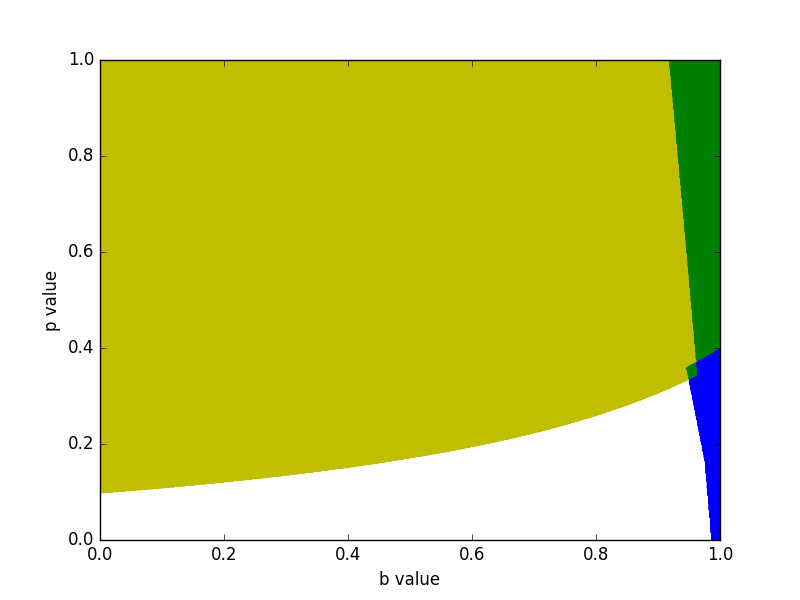
\includegraphics[height=2in]{\figurefolder/bp_pair_both_al0p5.png}
\caption{$\alpha = 0.5$}
\end{subfigure}%
~ 
\begin{subfigure}[t]{0.5\textwidth}
\centering
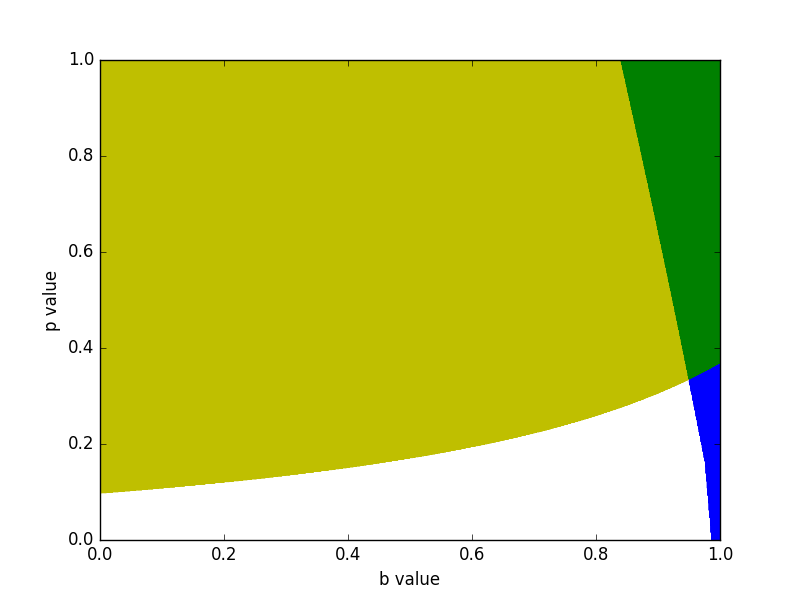
\includegraphics[height=2in]{\figurefolder/bp_pair_both_al1p0.png}
\caption{$\alpha = 1$}
\end{subfigure}
\centering
\begin{subfigure}[t]{0.5\textwidth}
\centering
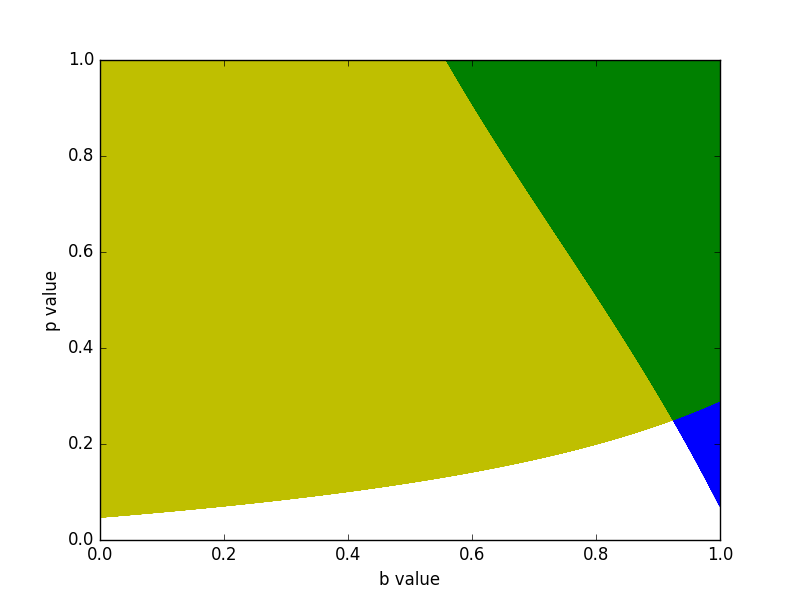
\includegraphics[height=2in]{\figurefolder/bp_pair_both_al2p0.png}
\caption{$\alpha = 2$}
\end{subfigure}%
~ 
\begin{subfigure}[t]{0.5\textwidth}
\centering
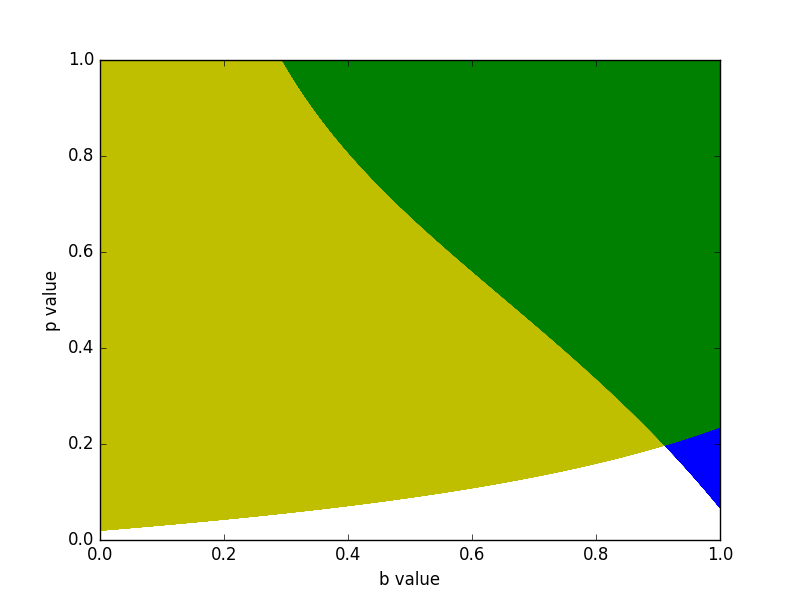
\includegraphics[height=2in]{\figurefolder/bp_pair_both_al2p5.png}
\caption{$\alpha = 2.5$}
\end{subfigure}

\caption{{Regions where $RoR_A > RoR_B$ (blue), where $RoR_A > \frac{b}{2}$ (yellow) and where both are true (green) for different values of $\alpha$. In all cases, $\beta = 0.95$ and $v = 0.05$.}}
\label{fig:offer_reward_or_not}
\end{figure*}

\begin{figure*}[t]
\centering
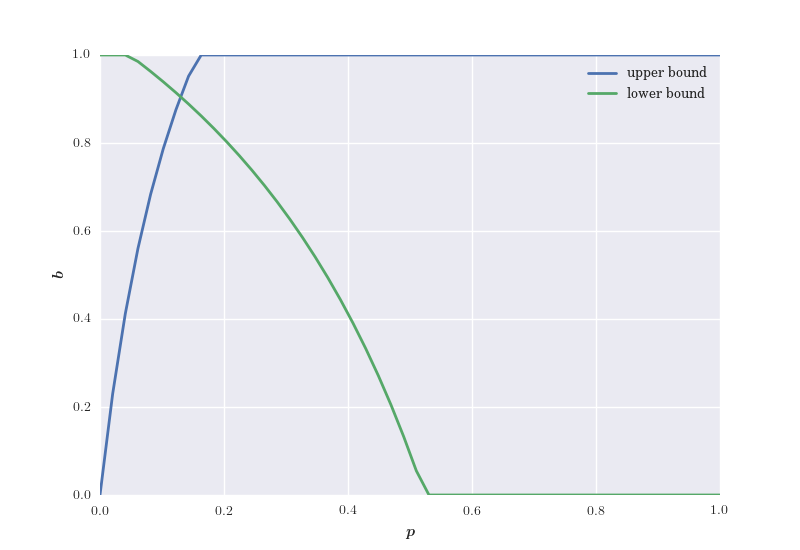
\includegraphics[scale = 0.6]{\figurefolder/b_region_v2.png}
\caption{The upper and lower bounds on $b$ as a function of $p$. Here $v = 0.05$ and $\alpha \rightarrow e$.}
\label{fig:b_region}
\end{figure*}

For any fixed $\alpha$, the exact conditions on $p$, $b$ and $v$ for $RoR_A > RoR_B$ and $RoR_A > \frac{b}{2}$ are rather complex. We will first focus on one particular simple case: $\alpha \rightarrow e$. 

\begin{lemma}
As $\alpha \rightarrow e$, $RoR_A > RoR_B$ if and only if the following condition on $b$ holds:
\begin{equation}
b > 2\cdot \frac{(1-v) - \frac{p}{1-p}\cdot (1-ev)}{(1-v) + (1-ev)}
\end{equation}
\end{lemma} 
\proof
First we compute the following quantity.
\begin{equation*}
\lim_{\alpha \to e} \frac{e-\alpha}{b\alpha}\log{1+\frac{b\alpha}{e-\alpha}}
\end{equation*}
Let $\frac{e-\alpha}{b\alpha} = x$, then it is easy to see that the above limit is equivalent to $\lim_{x\to \infty} \frac{\log(1+x)}{x} = 0$. Then as $\alpha \rightarrow e$, we have the following expressions for $RoR_A$ and $RoR_B$.
\begin{equation*}
RoR_A = (1-ev)\left(p+(1-p)\frac{b}{2} \right)
\end{equation*}
\begin{equation*}
RoR_B = (1-v)(1-p)\left(1-\frac{b}{2} \right)
\end{equation*}
And our condition $RoR_A > RoR_B$ simplifies.
\begin{align*}
(1-ev)\left(p+(1-p)\frac{b}{2} \right) &> (1-v)(1-p)\left(1-\frac{b}{2} \right) \\
\frac{b}{2}(1-p)(1-ev+1-v) &> (1-v)(1-p)-(1-ev)p \\
b &> 2\cdot \frac{(1-v) - \frac{p}{1-p}\cdot (1-ev)}{(1-v) + (1-ev)} 
\end{align*}

\endproof

The above lemma gives a lower bound on $b$ for $RoR_A > RoR_B$ in terms of $p$ and $v$. In order for the reward program to be strictly better than the traditional pricing model, we also need $RoR_A > \frac{b}{2}$. The following lemma shows that this condition gives a corresponding upper bound on $b$.

\begin{lemma}
As $\alpha \rightarrow e$, $RoR_A > \frac{b}{2}$ if and only if the following condition on $b$ holds:
\begin{equation}
b < \frac{2p}{p+\frac{ev}{1-ev}}
\end{equation}
\end{lemma} 

\proof
The condition $RoR_A > \frac{b}{2}$ is equivalent to:
\begin{align*}
(1-\alpha v)\left(p \frac{e}{\alpha}\left(1-\frac{e-\alpha}{b\alpha}\log \left(1+\frac{b\alpha}{e-\alpha} \right) \right)+(1-p)\frac{b}{2}\right) &> \frac{b}{2} \\
\frac{e}{\alpha} \left(1-\frac{e-\alpha}{b\alpha}\log \left(1+\frac{b\alpha}{e-\alpha} \right) \right) &> \frac{b}{2p}\left(\frac{1}{1-\alpha v}-(1-p) \right)
\end{align*}
As $\alpha \rightarrow e$, the left term above approaches 1 and we are left with:
\begin{align*}
b &< \frac{2 p (1-ev)}{1-(1-p)(1-ev)} \\
&= \frac{2p(1-ev)}{p-pev+ev} \\
&= \frac{2p}{p+\frac{ev}{1-ev}}
\end{align*}
\endproof

We combine the above two lemmas to get an intuitive necessary and sufficient condition on $p$ for the reward program to be ``strictly better''. 

\begin{lemma}
As $\alpha \rightarrow e$, for the reward program to be strictly better on some values of $b$, a necessary and sufficient condition on $p$ is:
\beq
\label{eq:necp}
p > 1 - \frac{1-ev}{1-ev^2}
\eeq
\end{lemma}

\proof
The previous two lemmas provide lower and upper bounds on $b$ for $RoR_A > RoR_B$ and $RoR_A > \frac{b}{2}$, respectively. For the reward program to be strictly better than all alternatives, both of these conditions must be met. The values of $b$ for which both are met is given by:
\begin{align*}
2\cdot \frac{(1-v) - \frac{p}{1-p}\cdot (1-ev)}{(1-v) + (1-ev)} < b < \frac{2p}{p+\frac{ev}{1-ev}}
\end{align*}
The above inequality is only valid when the lower bound is less than the upper bound. We may manipulate this inequality to get the simple condition on $p$ in our claim.
\begin{align*}
2\cdot \frac{(1-v) - \frac{p}{1-p}\cdot (1-ev)}{(1-v) + (1-ev)} &< \frac{2p}{p+\frac{ev}{1-ev}} \\
\left(p+\frac{ev}{1-ev} \right)\left((1-v)+\frac{p}{1-p}(1-ev) \right) &<  p(1-v+1-ev) \\
(1-v)\frac{ev}{1-ev} &< p(1-ev)+\frac{p^2}{1-p}(1-ev) + \frac{p}{1-p}ev \\
(1-p)(1-v)\frac{ev}{1-ev} &< (1-p)p(1-ev)+p^2(1-ev)+pev \\
(1-v)\frac{ev}{1-ev} &< p\left(1+(1-v)\frac{ev}{1-ev} \right) \\
\frac{(1-v)ev}{(1-ev)+(1-v)ev} &< p \\
\frac{ev-ev^2}{1-ev^2} &< p \\
\frac{(1-ev^2)-(1-ev)}{1-ev^2} &< p \\
1-\frac{1-ev}{1-ev^2} &< p
\end{align*}
\endproof

Thus, for any choice of $v$, and $p$ obeying the above condition, the combination of the above lemmas gives an interval of $b$ values for which the reward program is the most profitable choice for the merchant. 
Figure~\ref{fig:b_region} shows the bounds on $b$ for varying values of $p$, keeping $v = 0.05$ fixed, and restricting the range of $b$ values in $[0,1]$. 
Notice that the upper bound on $b$ increases as a function of $p$ while the lower bound decreases with $p$, so the interval of $b$ values where the reward program is strictly better increases with $p$. 
We formalize this observation in the next lemma. 

\begin{lemma}
As $\alpha \rightarrow e$ and $p$ obeying Eq.~\ref{eq:necp}, as $p$ increases, the range of values of $b$ for which the reward program is strictly better increases.
\end{lemma}

\proof
We know that the range of $b$ values in which we are interested is given by the interval.
\begin{align*}
2\cdot \frac{(1-v) - \frac{p}{1-p}\cdot (1-ev)}{(1-v) + (1-ev)} < b < \frac{2p}{p+\frac{ev}{1-ev}}
\end{align*}
Because $p$ obeys eq.~\ref{eq:necp}, the above inequality is valid. We will show that the above upper bound increases with $p$ and the lower bound decreases with increasing $p$. Therefore, as $p$ increases, the interval of $b$ values for which the reward program grows. First consider the upper bound, $UB(p) = \frac{2p}{p+\frac{ev}{1-ev}}$.
\begin{align*}
UB'(p) = \frac{ev}{(1-ev)\left(p+\frac{ev}{1-ev} \right)^2} \geq 0, \mbox{ } \forall p
\end{align*}
Now we consider the lower bound, $LB(p) = 2\cdot \frac{(1-v) - \frac{p}{1-p}\cdot (1-ev)}{(1-v) + (1-ev)}$.
\begin{align*}
LB'(p) = -\frac{2(1-ev)}{(1-p)^2((1-v)+(1-ev))} \leq 0, \mbox{ } \forall p
\end{align*}
\endproof

Figure~\ref{fig:b_restrictions} shows the upper and lower bounds on $b$ for all valid pairs of $p$ and $v$ with $\alpha \rightarrow e$. 
The top plot shows the lower bound on $b$ and the bottom plot depicts the upper bound. 
For a particular $(p,v)$ pair, if the color on the top plot is darker than the corresponding color on the bottom plot, then this pair has a valid $b$ interval in which the reward program is strictly better. 
This figure also exhibits the increasing range of $b$ values with increasing $p$; for large values of $p$ and moderate values of $v$, we observe no restrictions on $b$ for the reward program to be strictly better. 
We combine all the above observations into the following theorem.

\begin{figure}[h!]
\begin{centering}
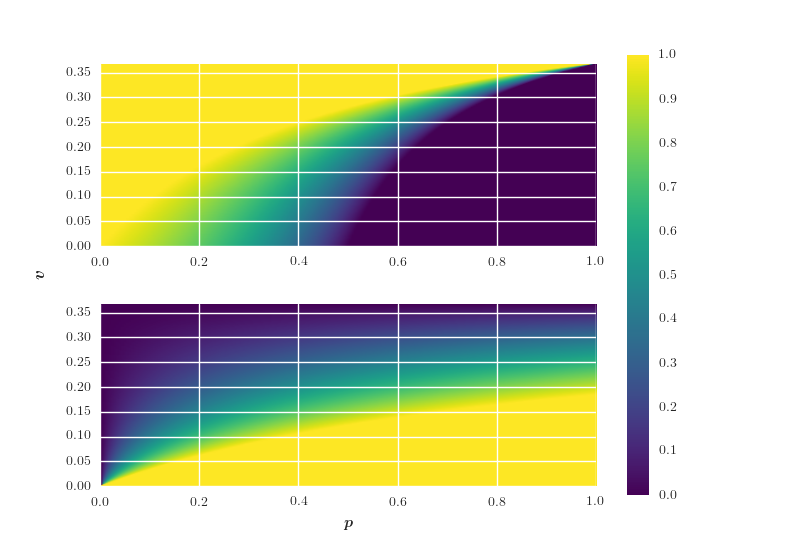
\includegraphics[scale = 0.75]{\figurefolder/b_bounds.png}
\caption{Bounds on $b$ for various values of $p$ and $v$ at $\alpha \rightarrow e$. Top shows lower bounds on $b$ for $RoR_A \geq RoR_B$ and bottom shows upper bounds of $b$ for $RoR_A \geq \frac{b}{2}$.}
\label{fig:b_restrictions}
\end{centering}
\end{figure}

\begin{theorem}
Under proportional budgeting, as $\alpha\rightarrow e$, a necessary and sufficient condition for reward program to be strictly better is a lowerbound on $p$ which increases with $v$.  
And as $p$ increases beyond the lowerbound, the region of allowable $b$ for which the reward program is strictly better becomes larger. 
\end{theorem}
%\proof
%\endproof

Now we generalize the above result for all values of $\alpha$. The conditions are more complex but the results and intuitions are similar. 

\begin{lemma}
Fix $\alpha \in (0, e)$. For any $(p,v)$ pair, there exists some upper bound $b_1 \in [0,1]$ such that for all $b \leq b_1$, $RoR_A \geq \frac{b}{2}$.
\end{lemma}

\proof
We delay the proof of this lemma to first prove a helpful proposition. It is a straightforward computation to see that the condition of $RoR_A \geq \frac{b}{2}$ is equivalent to:
\begin{gather*}
\frac{1}{b}\left(1-\frac{e-\alpha}{b\alpha}\log \left(1+\frac{b\alpha}{e-\alpha} \right) \right) \geq \frac{\alpha(1-(1-p)(1-\alpha v))}{2pe(1-\alpha v)} \\
\iff
g(b; \alpha) \geq h(p, v; \alpha)
\end{gather*}
where we have defined functions $g(b)$ and $h(p,v)$ for fixed $\alpha$ for the above inequalities. 

\begin{proposition}
For a fixed $\alpha$, $g(b)$ is non-increasing for all $b \in [0,1]$. 
\end{proposition}

\proof
We take the derivative of $g$:
\begin{align*}
g'(b) &= \frac{2(e-\alpha)}{b^3 \alpha} \log\left(1+\frac{b\alpha}{e-\alpha} \right) - \frac{1}{b^2}-\frac{1}{b^2\left(1+\frac{b\alpha}{e-\alpha}\right)} \leq 0 \\
&\iff \frac{2(e-\alpha)}{b \alpha} \log\left(1+\frac{b\alpha}{e-\alpha} \right) \leq 1+\frac{1}{1+\frac{b\alpha}{e-\alpha}} \\
&\iff \frac{2\log(1+x)}{x} \leq 1+\frac{1}{1+x}
\end{align*}
where $x = \frac{b\alpha}{e-\alpha}$, and as $b \in [0,1]$, $x \in [0, \frac{\alpha}{e-\alpha}]$. We can see that as $x \rightarrow 0$, the above inequality is an equality. 
We represent the LHS of the above equation as $L(x)$ and RHS as $R(x)$. Next we show that $L(x)$ increses slowly as compared to $R(x)$ thereby proving the proposition.
First show that in the range of $x$ the following holds true:

\beq
\label{eq:eq00}
\left(2-\frac{1}{1+x}\right)^2 \le 2\log(1+x) + 1
\eeq
To show the above observe that at $x\rightarrow 0$ both the LHS and RHS are equal. And it is easy to show that the derivative of LHS is lower than the derivative of RHS for all $x\ge 0$ as shown.
\begin{align*}
& (1+x) + \frac{1}{1+x} \ge 2\\
\implies & 2 - \frac{1}{1+x} \le 1 + x\\
\implies & (2-\frac{1}{1+x})\cdot \frac{1}{1+x} \le 1\\
\implies & 2\cdot(2-\frac{1}{1+x})\cdot (\frac{1}{1+x})^2 \le \frac{2}{1+x}
\end{align*}
The left hand side is the derivative of the above LHS and right hand side is the derivative of the above RHS.

Now we can rearrange Eq.~\ref{eq:eq00} as follows:
\begin{align*}
& \left(2-\frac{1}{1+x}\right)^2 \le 2\log(1+x) + 1\\
\implies & (1 + \frac{x}{1+x})^2 \le 2\log(1+x) + 1\\
\implies & (\frac{x}{1+x})^2 + \frac{2x}{1+x} \le 2\log(1+x)\\
\implies & 2\left(\frac{x}{1+x} - \log(1+x)\right) \le - (\frac{x}{1+x})^2\\
\implies & \frac{2\left(\frac{x}{1+x} - \log(1+x)\right)}{x^2} \le - (\frac{1}{1+x})^2
\end{align*}
The left hand side of above is $L'(x)$ and right hand side is $R'(x)$.

\endproof

Thus, $g(b)$ is decreasing in $b$, so for any $(p,v)$ pair, we may compute $h(p, v; \alpha)$, which will then fall into one of the following three cases.
\begin{itemize}
\item
$h(p,v;\alpha) \geq g(0)$. So no value of $b$ makes the reward program profitable.
\item
$h(p,v;\alpha) \leq g(1)$. So any value of $b$ makes the reward program profitable.
\item
$h(p,v;\alpha) = g(b_0)$ for some $b_0 \in (0,1)$. So the reward program is profitable for all $b \leq b_0$ and not otherwise.
\end{itemize}

The above proposition and discussion proves our lemma: for fixed $\alpha$ and any $(p,v)$ pair, there is some upperbound on $b$ s.t. $RoR_A > \frac{b}{2}$. 
\endproof

Now we again look at the conditions for $RoR_A > RoR_B$ to get a lower bound on $b$.  
\begin{lemma}
Fix $\alpha \in (0, e)$. For any $(p,v)$ pair, there exists some lower bound $b_0 \in [0,1]$ such that for all $b \geq b_0$, $RoR_A > RoR_B$.
\end{lemma}

\proof
Let $\frac{b\alpha}{e-\alpha} = X$. Then $RoR_A > RoR_B$ can be evaluated as follows:

\begin{eqnarray}
& p\frac{e}{\alpha}\left(1-\frac{\log(1+X)}{X}\right)(1-\alpha v + 1 - v) - p(1-v) + (1-p)\frac{b}{2}\left(1-\alpha v + 1-v\right) + p(1-v) > 1-v\notag\\
& \implies p\left(1 - \frac{\log(1+X)}{X}\right) + (1-p)\frac{b\alpha}{2e} > \frac{\alpha}{e} \cdot \frac{1-v}{1-\alpha v + 1 - v}\label{eq:ra>rb}
\end{eqnarray}

Since $\alpha$ is a constant, the LHS above is a function of $b$ and $p$. 
Let the LHS above be $L(b,p)$.
We first show that in the range of $b\in [0,1]$, $1 - \frac{\log(1+X)}{X} > \frac{b\alpha}{2e}$ which shows that $L(b,p)$ is increasing in $p$.

\begin{align*}
& 1-\frac{\log(1+X)}{X} > \frac{b\alpha}{2e}\\
\Leftrightarrow & X - \log(1+X) > \frac{b^2\alpha^2}{2e(e-\alpha)}
\end{align*}
Observe that LHS is equal to RHS when $b\rightarrow 0$. 
All we show is that LHS increases faster than RHS in the range of $b\in [0,1]$. 

\begin{align*}
\Leftrightarrow & \left(1 - \frac{1}{1+X}\right) \frac{\alpha}{e-\alpha} > \frac{b\alpha^2}{e(e-\alpha)}\\
\Leftrightarrow & \frac{1}{1+X} > \frac{e-\alpha}{e}\\
\Leftrightarrow & \frac{e}{e-\alpha} > 1 + \frac{b\alpha}{e-\alpha}
\end{align*}
And the last equation is true in the range of $b\in [0,1]$. Hence $L(b,p)$ increases with $p$.

Now we show that $L(b,p)$ increases with $b$ as well. First observe:

\beq
\frac{\partial L(b,p)}{\partial b} = p\left(\frac{\log(1+X) - \frac{X}{1+X}}{X^2}\right)\frac{\alpha}{e-\alpha} + (1-p)\frac{\alpha}{2e}
\notag
\eeq

Thus $\frac{\partial L(b,p)}{\partial b} > 0$ implies:

\begin{align*}
& (1-p)\frac{\alpha}{2e} > p\left(\frac{\frac{X}{1+X} - \log(1+X)}{X^2}\right)\frac{\alpha}{e-\alpha}\\
\Leftrightarrow & (1-p)\frac{b^2\alpha^2}{2e(e-\alpha)} > p \left(1 - \frac{1}{1+X} - \log(1+X)\right)
\end{align*}

Again the LHS and RHS are equal as $b\rightarrow 0$. All we show again is that LHS increases faster as compared to RHS.

\begin{align*}
\Leftrightarrow (1-p)\frac{b\alpha^2}{e(e-\alpha)} > p\left(\frac{1}{(1+X)^2} - \frac{1}{1+X} \right)\frac{\alpha}{e-\alpha}\\
\end{align*}
Clearly RHS is negative when $b\in (0,1]$ and LHS is positive. Hence proved.

Thus $L(b,p)$ is increasing in both $b$ and $p$. And the condition required is $L(b,p)$ is greater than some constant value which depends on $v$.
Hence for any $v$ there exists a smooth $(b_0,p_0)$ curve such that for all $b\ge b_0$ and $p\ge p_0$ revenue rate of reward program merchant is larger.

\endproof

We combine the above two lemmas as before to get the following theorem.

\begin{theorem}
Fix $\alpha \in (0, e)$. 
For any value of $v$, there exists a lowerbound $p_0$ such that for any $p$ greater than $p_0$, there exists a range $(b_0, b_1)$ between $0$ and $1$ such that for all $b$ lying between $b_0$ and $b_1$, offering the reward program is strictly better for $A$. 
\end{theorem}

The above results can be extremely helpful in the following way: if a merchant has good estimates of its target customer population, \ie, $b$ and $p$ values, it can find the appropriate reward budget ratios $\alpha$, which could make running a reward program strictly better against a traditional pricing competitor.


\section{Conclusions}
\label{sec:conc}
We investigated the optimal design of a frequency reward program against traditional pricing in a competitive duopoly.
We modeled the behavior of customers valuing their utility in rational economic terms, and our theoretical results agree with past empirical studies.
Assuming general distributions of customer population, we characterized optimal parameters for the design of reward program, and under more specific parameter distrubution assumptions, we showed the conditions on customer population parameters which make the reward program strictly better.
In short, if a merchant can make good estimates of the customer population parameters, our model and results can help understand the pros and cons of running a frequency reward program for that merchant against traditional pricing.

Though our research offers some interesting managerial insights, there are some limitations to our study. 
Our results on revenue comparisons assumed specific distributions for the customer population, though our framework can be extended to other distributions as well. Moreover, estimating the customer population distribution and parameters using real transactional data is an interesting question in itself.
That is, backing this research with empirical and experimental study, could provide strong quantifications to the intuitions we discuss.
We modeled customer behavior in rational economic terms, mainly to understand the rational components that affect the decision making process.
Tying in the effects of our research with some past models on psychological behavior patterns of customers toward reward programs would be another practically relevant problem to address.
Finally, we modeled a competitive duopoly, but left the traditional pricing merchant as non-strategic.
Understanding how competition affects the equilibrium prices and reward program parameters could give intuitions about a more practical scenario. 



\bibliographystyle{plainnat}
\setcitestyle{numbers}
\bibliography{\basefolder/bibliography}

\end{document}
